% Results section: exp / sepalpha / commem / TK, after screening out top-endpoint responders.
% Estimates: python run_exclusion_check.py --pw tk --lambda-upper 20 --gamma-lower 0.28 --test2 \
%   --output-dir results_grid_conditional_stricter_no_endpoint_tk_main  (see the script docstring)
% Figures: python slides/make_figures.py  (writes slides/figures/*.pdf)
% Compile: pdflatex results.tex  (run inside slides/)
\documentclass[aspectratio=169,11pt]{beamer}

\usepackage[T1]{fontenc}
\usepackage{lmodern}
\usepackage{amsmath,amssymb}
\usepackage{booktabs}
\usepackage{graphicx}

\definecolor{accent}{HTML}{2A78D6}
\definecolor{ink}{HTML}{0B0B0B}
\definecolor{muted}{HTML}{52514E}

\usetheme{default}
\setbeamertemplate{navigation symbols}{}
\setbeamertemplate{footline}[frame number]
\setbeamertemplate{itemize items}[circle]
\setbeamercolor{normal text}{fg=ink}
\setbeamercolor{structure}{fg=accent}
\setbeamercolor{frametitle}{fg=ink}
\setbeamercolor{title}{fg=ink}
\setbeamercolor{subtitle}{fg=muted}
\setbeamerfont{frametitle}{series=\bfseries}
\setbeamerfont{title}{series=\bfseries}

\graphicspath{{figures/}}

\newcommand{\ap}{\alpha^{+}}
\newcommand{\am}{\alpha^{-}}
\newcommand{\bd}{\ensuremath{^{\dagger}}}
\newcommand{\tabnote}[1]{\par\vfill{\scriptsize\color{muted}#1\par}}
\newcommand{\tight}{\setlength{\itemsep}{3pt}}

\title{Estimation Results}
\subtitle{Exponential discounting $\cdot$ separate curvature $\cdot$ common memory decay $\cdot$ Tversky--Kahneman weighting}
\date{}

\begin{document}

\begin{frame}
  \titlepage
\end{frame}

% ---------------------------------------------------------------------------
\begin{frame}{Specification and sample}
\begin{columns}[T,onlytextwidth]
\begin{column}{0.55\textwidth}
\textbf{Specification (fixed throughout)}
\begin{itemize}\small\tight
  \item Value: $(x-R)^{\ap}$ for gains, $-\lambda(R-x)^{\am}$ for losses
  \item Delayed payments discounted by $e^{-rt}$ (exponential, $\psi=1$)
  \item Rank-dependent TK weighting $w(p)=\dfrac{p^{\gamma}}{\big(p^{\gamma}+(1-p)^{\gamma}\big)^{1/\gamma}}$, $\gamma\ge 0.28$ (monotone)
  \item $R_t=a_{SQ}R^{SQ}+a_{PA}R^{A}_t+a_{LE}R^{LE}_t+a_{FE}R^{FE}_t$; one memory decay $\delta$ drives both $R^{A}$ and $R^{LE}$
  \item Loss aversion reported as $A(x)=\lambda x^{\am-\ap}$: loss vs.\ gain value of $\pm$\pounds$x$
\end{itemize}
\end{column}
\begin{column}{0.41\textwidth}
\textbf{Three tests}
\begin{itemize}\small\tight
  \item \textbf{Test 1:} $C$ latent classes, RP weights free in each class
  \item \textbf{Test 2:} one class, one pure RP (SQ, PA, LE or FE)
  \item \textbf{Test 3:} four classes, each pinned to one pure RP
\end{itemize}
\vspace{6pt}
\textbf{Data and estimation}
\begin{itemize}\small\tight
  \item 851 participants, 15{,}317 CEs after screening (next slides)
  \item EM, 100 random + warm starts per model; $\lambda\le 20$
\end{itemize}
\end{column}
\end{columns}
\end{frame}

% ---------------------------------------------------------------------------
\begin{frame}{Screening: participants who answer at the top of the list}
\begin{columns}[c,onlytextwidth]
\begin{column}{0.52\textwidth}
\centering
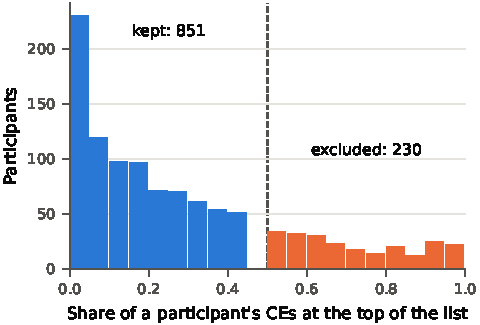
\includegraphics[width=\linewidth]{screening.pdf}
\end{column}
\begin{column}{0.45\textwidth}
\begin{itemize}\small\tight
  \item \textbf{Top-of-list answer:} keep the lottery until the sure amount equals its best outcome, so the CE is the best outcome
  \item 27.6\% of all 19{,}457 CEs are top-of-list answers
  \item \textbf{Rule:} exclude participants with at least half of their CEs at the top
  \item \textbf{Excluded: 230 of 1{,}081 participants (21\%)}, 4{,}140 CEs; 851 participants and 15{,}317 CEs remain
  \item Occasional top answers stay: 621 of the 851 kept participants give 1--8 (15.6\% of kept CEs)
\end{itemize}
\end{column}
\end{columns}
\tabnote{List length differs across lotteries (9 to 20 rows), so the top is identified by the amount (= best remaining outcome), not by the row number.}
\end{frame}

% ---------------------------------------------------------------------------
\begin{frame}{Who are the excluded participants?}
{\centering\footnotesize
\begin{tabular}{l rr}
\toprule
& Excluded (230) & Kept (851)\\
\midrule
CEs at the top of the list & \textbf{72\%} & 16\%\\
\quad when the best outcome has $p\le 0.25$ & 69\% & 12\%\\
\quad when the best outcome has $p>0.75$ & 75\% & 23\%\\
\quad in gain / loss / mixed lotteries & 72 / 78 / 61\% & 15 / 22 / 5\%\\
\quad in sessions 1 / 2 / 3 (different days) & 72 / 71 / 76\% & 15 / 24 / 24\%\\
Other CEs track the EV (median within-person corr.) & 0.05 & 0.16\\
\midrule
Rated the study ``not complicated at all'' ($p<0.001$) & 16\% & 27\%\\
Any failed comprehension attempt ($p=0.02$) & 47\% & 38\%\\
``Paid attention throughout'' ($p=0.35$) & 93\% & 94\%\\
University degree ($p=0.08$) & 64\% & 70\%\\
\midrule
Full-sample Test 3 type: FE / LE / SQ / PA & 165 / 40 / 17 / 8 & \\
\bottomrule
\end{tabular}\par}
\begin{itemize}\small\tight
  \item A response rule that ignores the lottery (56--87\% in each of the 16 lotteries); in the full sample it produced the ``FE'' corner type ($\ap=5$, $\lambda\approx 6$)
\end{itemize}
\tabnote{$p$-values: $\chi^2$ test (complexity) and Fisher exact tests.}
\end{frame}

% ---------------------------------------------------------------------------
\begin{frame}{Model fit (screened sample)}
{\centering\footnotesize
\begin{tabular}{cl rrrrr}
\toprule
Test & Model & $k$ & Log-lik. & BIC & $\Delta$BIC & median $\xi_i$\\
\midrule
2 & Pure SQ & 5 & $-71{,}665.4$ & 151{,}579.8 & 2{,}138.2 & 0.254\\
2 & Pure PA & 6 & $-71{,}653.6$ & 151{,}566.0 & 2{,}124.4 & 0.254\\
2 & Pure LE & 6 & $-71{,}669.1$ & 151{,}596.8 & 2{,}155.3 & 0.255\\
2 & Pure FE & 5 & $-71{,}837.4$ & 151{,}923.7 & 2{,}482.2 & 0.259\\
\midrule
1 & $C=1$, free RP mix & 9 & $-71{,}649.1$ & 151{,}585.8 & 2{,}144.2 & 0.254\\
1 & $C=2$ & 19 & $-71{,}004.9$ & 150{,}393.7 & 952.1 & 0.235\\
1 & $C=3$ & 29 & $-70{,}699.1$ & 149{,}878.5 & 437.0 & 0.225\\
1 & $C=4$ & 39 & $\mathbf{-70{,}453.6}$ & 149{,}484.0 & 42.4 & 0.221\\
\midrule
3 & SQ / PA / LE / FE types & 25 & $-70{,}499.9$ & \textbf{149{,}441.6} & \textbf{0} & 0.225\\
\bottomrule
\end{tabular}\par}
\begin{itemize}\small\tight
  \item Four classes vs.\ one: $+1{,}195$ log-lik.; choice of a pure RP for one agent: $\le 184$
  \item Test 3 has the lowest BIC: $46.3$ log-lik.\ below Test 1 ($C=4$) with 14 fewer parameters
  \item $C=5,6$ lower the BIC further but only by adding degenerate classes (backup)
\end{itemize}
\tabnote{$k$: structural parameters and mixing weights; the 851 noise parameters $\xi_i$ also enter the BIC. $n=15{,}317$.}
\end{frame}

% ---------------------------------------------------------------------------
\begin{frame}{One representative agent ($C=1$)}
{\centering\footnotesize
\begin{tabular}{l rrrr r}
\toprule
& \multicolumn{4}{c}{Test 2: pure reference point} & Test 1\\
\cmidrule(lr){2-5}
& SQ & PA & LE & FE & free mix\\
\midrule
Log-lik. & $-71{,}665.4$ & $\mathbf{-71{,}653.6}$ & $-71{,}669.1$ & $-71{,}837.4$ & $-71{,}649.1$\\
$\ap$ & 1.058 & 1.062 & 1.058 & 1.159 & 1.040\\
$\am$ & 0.951 & 0.961 & 0.932 & 1.266 & 0.947\\
$\lambda$ & 1.831 & 1.792 & 1.985 & 0.525 & 1.729\\
$A(20)$ & 1.33 & 1.33 & 1.36 & 0.72 & 1.31\\
$\gamma$ & 0.595 & 0.593 & 0.600 & 0.349 & 0.594\\
$\delta$ & -- & 0.890 & 1.000\bd & -- & 0.444\\
RP weights & & & & & $(.00,.78,.00,.22)$\\
\bottomrule
\end{tabular}\par}
\begin{itemize}\small\tight
  \item SQ, PA, LE: same preferences ($\ap\approx 1.06$, $\am\approx 0.95$, $\gamma\approx 0.6$, $A(20)\approx 1.33$)
  \item PA fits best; FE is clearly worst ($-184$) and the only RP with $A<1$
  \item The free mix (PA $0.78$ + FE $0.22$) gains only $4.6$ log-lik.\ over pure PA (BIC $+20$)
\end{itemize}
\tabnote{\bd\ at a bound. $r$ at its lower bound except under pure FE (0.019). RP weights: SQ, PA, LE, FE.}
\end{frame}

% ---------------------------------------------------------------------------
\begin{frame}{Test 1: four latent classes with free reference-point weights}
\begin{columns}[T,onlytextwidth]
\begin{column}{0.47\textwidth}
\centering\footnotesize\setlength{\tabcolsep}{4pt}
\begin{tabular}{l rrrr}
\toprule
Class & 1 & 2 & 3 & 4\\
Share $\pi$ & 38.9\% & 26.0\% & 22.8\% & 12.3\%\\
\midrule
$a_{SQ}$ & 0.010 & 0.004 & 0.169 & 0.228\\
$a_{PA}$ & 0.308 & 0.000 & 0.195 & \textbf{0.772}\\
$a_{LE}$ & 0.307 & 0.042 & 0.358 & 0.000\\
$a_{FE}$ & 0.374 & \textbf{0.954} & 0.277 & 0.000\\
$\delta$ & 1.000\bd & 0.200\bd & 0.952 & 0.689\\
\midrule
$\ap$ & 1.136 & 1.634 & 1.003 & 1.035\\
$\am$ & 0.674 & 1.765 & 0.954 & 1.176\\
$\lambda$ & 6.850 & 0.934 & 1.353 & 0.688\\
$\gamma$ & 0.555 & 0.305 & 0.893 & 0.280\bd\\
$A(5)$ & 3.26 & 1.15 & 1.25 & 0.86\\
$A(20)$ & 1.72 & 1.38 & 1.17 & 1.05\\
$A(50)$ & 1.12 & 1.56 & 1.12 & 1.19\\
\bottomrule
\end{tabular}
\end{column}
\begin{column}{0.49\textwidth}
\begin{itemize}\small\tight
  \item \textbf{Two pure-RP classes:} FE (class 2, 26\%) and PA (class 4, 12\%, with some SQ)
  \item \textbf{Two mixed-RP classes} without a dominant reference point (largest weight $0.37$):
  \begin{itemize}\footnotesize
    \item Class 1 (39\%): loss aversion at small stakes ($A(5)=3.3$, $A(50)=1.1$)
    \item Class 3 (23\%): close to expected value ($\alpha^{\pm}\approx 1$, $\gamma=0.89$)
  \end{itemize}
  \item Population RP weights: SQ $0.07$, PA $0.26$, LE $0.21$, FE $0.46$
\end{itemize}
\end{column}
\end{columns}
\tabnote{\bd\ at an estimation bound ($\delta$ only matters where $a_{PA}$ or $a_{LE}>0$; $\gamma\ge 0.28$ keeps TK monotone). $r$ is at its lower bound in all classes.}
\end{frame}

% ---------------------------------------------------------------------------
\begin{frame}{Test 3: four pure reference-point types (lowest BIC)}
\begin{columns}[T,onlytextwidth]
\begin{column}{0.45\textwidth}
\centering\footnotesize\setlength{\tabcolsep}{4pt}
\begin{tabular}{l rrrr}
\toprule
Type & SQ & PA & LE & FE\\
\midrule
Share $\pi$ & 19.1\% & 13.7\% & \textbf{39.5\%} & 27.7\%\\
Modal $n$ & 142 & 115 & 347 & 247\\
\midrule
$\ap$ & 0.995 & 1.069 & 1.202 & 1.585\\
$\am$ & 0.940 & 1.187 & 0.483 & 1.777\\
$\lambda$ & 1.385 & 0.785 & 20.000\bd & 0.620\\
$\gamma$ & 0.942 & 0.287 & 0.563 & 0.283\\
$\delta$ & -- & 1.000\bd & 1.000\bd & --\\
$A(5)$ & 1.27 & 0.95 & \textbf{6.29} & 0.84\\
$A(20)$ & 1.17 & 1.11 & 2.32 & 1.10\\
$A(50)$ & 1.12 & 1.24 & 1.20 & 1.31\\
\bottomrule
\end{tabular}
\end{column}
\begin{column}{0.51\textwidth}
\begin{itemize}\small\tight
  \item \textbf{LE} (40\%): loss aversion concentrated at small stakes ($A=6.3$ at \pounds 5, $1.2$ at \pounds 50); $\lambda$ hits its bound because it trades off with $\am$, so read $A(x)$, not $\lambda$
  \item \textbf{SQ} (19\%): close to expected value ($\alpha^{\pm}\approx 1$, $\gamma=0.94$)
  \item \textbf{PA} (14\%) and \textbf{FE} (28\%): the strongest probability insensitivity TK allows ($\gamma\approx 0.28$); FE has curvature above 1 on both sides
  \item Sharp classification: mean maximum posterior 0.85; 96\% above 0.5
\end{itemize}
\end{column}
\end{columns}
\tabnote{\bd\ at an estimation bound. $\delta$ is not identified for the SQ and FE types; $r$ is at its lower bound for all types.}
\end{frame}

% ---------------------------------------------------------------------------
\begin{frame}{What the Test 3 types do in the data}
{\centering\footnotesize
\begin{tabular}{l r r rrrr}
\toprule
& & & \multicolumn{4}{c}{Mean CE position, by modal type}\\
\cmidrule(lr){4-7}
Remaining lottery & CEs & EV & SQ & PA & LE & FE\\
\midrule
Gains only & 5{,}693 & 0.68 & 0.70 & \textbf{0.25} & 0.57 & 0.51\\
Mixed & 3{,}731 & 0.50 & 0.51 & 0.38 & 0.57 & 0.42\\
Losses only & 5{,}893 & 0.60 & 0.61 & \textbf{0.81} & 0.73 & 0.46\\
\midrule
\multicolumn{3}{l}{Corr.\ of CE with EV across lotteries} & \textbf{0.55} & $-0.12$ & 0.12 & 0.24\\
\multicolumn{3}{l}{Share in top 10\% of range} & 0.18 & 0.23 & 0.24 & 0.08\\
\bottomrule
\end{tabular}\par}
\begin{itemize}\small\tight
  \item \textbf{SQ:} CEs at the EV in every domain and they move with the EV across lotteries
  \item \textbf{PA:} extreme reflection (low CEs for gains, high for losses) that ignores the EV
  \item \textbf{LE:} risk averse over gains, risk seeking over losses; \textbf{FE:} below the EV everywhere
\end{itemize}
\tabnote{CE position $=(CE-\min)/(\max-\min)$ over the undiscounted payoffs of the remaining lottery; the EV column gives the same position for the expected value. Correlation: median within-person correlation of CE and EV positions.}
\end{frame}

% ---------------------------------------------------------------------------
\begin{frame}{Same participants, two descriptions: Test 1 ($C=4$) vs.\ Test 3}
\begin{columns}[c,onlytextwidth]
\begin{column}{0.52\textwidth}
\centering
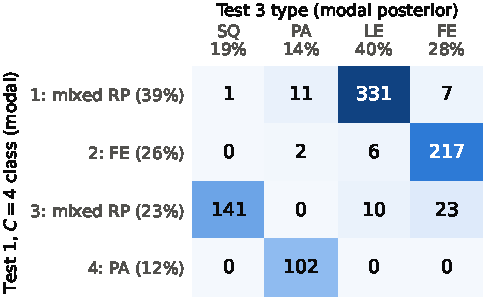
\includegraphics[width=\linewidth]{crosstab_test1_test3.pdf}
\end{column}
\begin{column}{0.45\textwidth}
\begin{itemize}\small\tight
  \item \textbf{The four groups match:} 93\% of participants (791 of 851) fall in the corresponding class and type
  \item \textbf{FE and PA} are pure reference points in both tests
  \item \textbf{LE and SQ} correspond to mixed-RP classes when weights are free, so these two labels come from the pure-type restriction, not from the data
\end{itemize}
\end{column}
\end{columns}
\tabnote{Counts of participants by modal posterior class in each model; $n=851$. Classes numbered by share, as on the Test 1 slide.}
\end{frame}

% ---------------------------------------------------------------------------
\begin{frame}{Robustness: Prelec vs.\ TK weighting (same screened sample)}
{\centering\footnotesize
\begin{tabular}{l rr}
\toprule
& Prelec & TK\\
\midrule
BIC, Test 3 & 149{,}484.0 & \textbf{149{,}441.6}\\
BIC, Test 1 ($C=4$) & 149{,}513.8 & 149{,}484.0\\
Same Test 3 type under both & \multicolumn{2}{c}{775 of 851 (91\%)}\\
\midrule
$A(20)$: SQ / PA / LE / FE & 1.17 / 1.20 / 2.10 / 1.37 & 1.17 / 1.11 / 2.32 / 1.10\\
Weighting parameter: PA / FE & $0^{\dagger}$ / $0^{\dagger}$ & 0.287 / 0.283\\
\bottomrule
\end{tabular}\par}
\begin{itemize}\small\tight
  \item TK fits better after screening (BIC $-42$ for Test 3); in the full sample Prelec was ahead by 30, so its advantage came from the top-of-list group
  \item Type membership and $A(20)$ hardly change with the weighting function
  \item PA and FE types: Prelec $\gamma\to 0$ and TK's monotonicity limit describe the same strong probability insensitivity
\end{itemize}
\tabnote{\bd\ at an estimation bound. Both fits use $\lambda\le 20$; Prelec weighting parameter $\alpha$ in $w(p)=\exp[-(-\ln p)^{\alpha}]$.}
\end{frame}

% ---------------------------------------------------------------------------
\begin{frame}{Takeaways}
\begin{enumerate}\tight
  \item \textbf{Screening.} 21\% of participants answer at the top of the choice list in about 72\% of decisions, whatever the lottery; they formed the full-sample ``FE'' corner type and are excluded.
  \item \textbf{Heterogeneity is first order.} Four classes gain $\approx 1{,}200$ log-likelihood points over one; the choice of a single pure RP moves the fit by at most 184.
  \item \textbf{Four robust groups.} The same participants form them in Test 1 and Test 3 (93\%) and under Prelec and TK (91\%).
  \item \textbf{Reference points.} The FE (28\%) and PA (14\%) groups use one pure reference point in both tests; the LE (40\%) and SQ (19\%) labels are not supported once weights are free.
  \item \textbf{Preferences.} Loss aversion is modest at \pounds 20 ($A\approx 1.1$--$2.3$) and strongest for the LE group at small stakes; PA and FE are strongly probability insensitive; the SQ group behaves close to expected value.
\end{enumerate}
\end{frame}

% ===========================================================================
\appendix

\begin{frame}{Backup: why four classes}
{\centering\footnotesize
\begin{tabular}{l rrrr}
\toprule
Model & BIC & ICL & Smallest class & Posterior $>0.9$\\
\midrule
Test 1, $C=1$ & 151{,}585.8 & 151{,}585.8 & 100\% & 100\%\\
Test 1, $C=2$ & 150{,}393.7 & 150{,}538.3 & 19.5\% & 88\%\\
Test 1, $C=3$ & 149{,}878.5 & 150{,}215.0 & 17.2\% & 75\%\\
Test 1, $C=4$ & 149{,}484.0 & 150{,}093.6 & 12.3\% & 56\%\\
Test 1, $C=5$ & 149{,}296.6 & 150{,}003.6 & 7.0\% & 52\%\\
Test 1, $C=6$ & 149{,}171.4 & 150{,}000.6 & 6.8\% & 44\%\\
\midrule
Test 3 & 149{,}441.6 & 150{,}070.8 & 13.7\% & 56\%\\
\bottomrule
\end{tabular}\par}
\begin{itemize}\small\tight
  \item BIC keeps falling; ICL (BIC $+\,2\times$ classification entropy) flattens at $C=5$--$6$
  \item The extra classes are degenerate: $\ap\to 0$ for 7\% of participants, $\lambda$ at its bound of 20 or $\lambda=0.04$, and $\gamma$ at 0.28 in 3 of 6 classes
  \item $C=4$: every class is interpretable and matches a Test 3 type
\end{itemize}
\tabnote{$C=5,6$ were started from every class of the $C-1$ fit split in two, plus 100 random starts.}
\end{frame}

\begin{frame}{Backup: optimisation diagnostics}
{\centering\footnotesize
\begin{tabular}{l ccc c}
\toprule
& \multicolumn{3}{c}{Starts within $x$ of the best log-lik.} & \\
\cmidrule(lr){2-4}
Model & $x=0.01$ & $x=1$ & $x=10$ & Starts\\
\midrule
Test 2 (each RP) & 83--101 & 101 & 101 & 101\\
Test 1, $C=1$ & 1 & 24 & 71 & 102\\
Test 1, $C=2$ & 1 & 1 & 7 & 103\\
Test 1, $C=3$ & 2 & 2 & 4 & 104\\
Test 1, $C=4$ & 1 & 2 & 13 & 107\\
Test 3 & 6 & 6 & 11 & 102\\
\bottomrule
\end{tabular}\par}
\begin{itemize}\small\tight
  \item All fits converged (log-lik.\ change $<10^{-6}$); the mixture likelihoods are multimodal, so a global optimum is not guaranteed
  \item Warm starts: full-sample fit, earlier screened fits, nested Test 3 fit (for $C=4$), split $C-1$ classes
  \item At bounds: $r$ everywhere (no detectable discounting), $\delta$ in several classes, $\gamma=0.28$ (Test 1 class 4), $\lambda=20$ (LE type)
\end{itemize}
\end{frame}

\begin{frame}{Backup (full sample, Prelec): profile likelihood of $\lambda$, PA type}
\begin{columns}[c,onlytextwidth]
\begin{column}{0.52\textwidth}
\centering
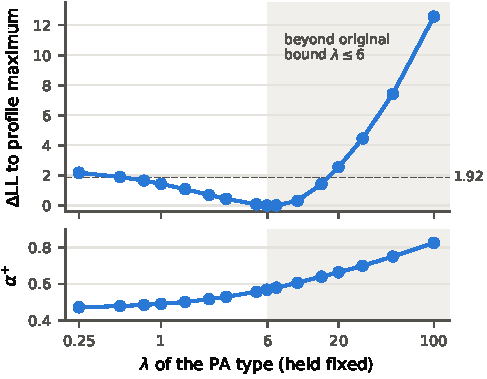
\includegraphics[width=\linewidth]{profile_lambda.pdf}
\end{column}
\begin{column}{0.45\textwidth}
\begin{itemize}\small\tight
  \item Before screening, Prelec specification: $\lambda$ fixed on a grid, all other parameters, shares and $\xi_i$ re-estimated
  \item Very flat: $\Delta$LL $\le 2.6$ on $[0.25,20]$; the maximum is at $\lambda\approx 6$--$7$
  \item $\lambda$ trades off against $\ap$, which is why the slides report $A(x)$ instead of $\lambda$
\end{itemize}
\end{column}
\end{columns}
\tabnote{Dashed line: $1.92=\chi^2_{1,0.95}/2$, a heuristic only (nuisance parameters on the boundary, mixture model).}
\end{frame}

\begin{frame}{Backup (full sample, Prelec): profile likelihood of $\gamma$, PA type}
\begin{columns}[c,onlytextwidth]
\begin{column}{0.52\textwidth}
\centering
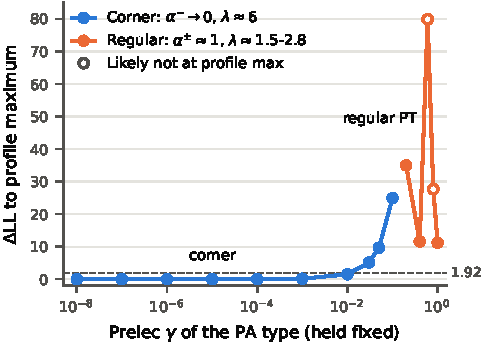
\includegraphics[width=\linewidth]{profile_gamma.pdf}
\end{column}
\begin{column}{0.45\textwidth}
\begin{itemize}\small\tight
  \item Flat for $\gamma\le 10^{-3}$, then steep ($\Delta$LL 1.5 at 0.01, 25 at 0.1): the PA type's probability insensitivity is not a numerical artefact
  \item Under TK the same group sits at the monotonicity limit $\gamma\approx 0.28$
  \item For $\gamma\ge 0.2$ only 1--3 of 12 starts reach the best value, so $\Delta$LL there is an upper bound
\end{itemize}
\end{column}
\end{columns}
\tabnote{Hollow points: non-monotone values reached by a single start.}
\end{frame}

\end{document}
